\PassOptionsToPackage{table}{xcolor}
\documentclass{book}\usepackage[]{graphicx}\usepackage[]{color}
% maxwidth is the original width if it is less than linewidth
% otherwise use linewidth (to make sure the graphics do not exceed the margin)
\makeatletter
\def\maxwidth{ %
  \ifdim\Gin@nat@width>\linewidth
    \linewidth
  \else
    \Gin@nat@width
  \fi
}
\makeatother

\definecolor{fgcolor}{rgb}{0.345, 0.345, 0.345}
\newcommand{\hlnum}[1]{\textcolor[rgb]{0.686,0.059,0.569}{#1}}%
\newcommand{\hlstr}[1]{\textcolor[rgb]{0.192,0.494,0.8}{#1}}%
\newcommand{\hlcom}[1]{\textcolor[rgb]{0.678,0.584,0.686}{\textit{#1}}}%
\newcommand{\hlopt}[1]{\textcolor[rgb]{0,0,0}{#1}}%
\newcommand{\hlstd}[1]{\textcolor[rgb]{0.345,0.345,0.345}{#1}}%
\newcommand{\hlkwa}[1]{\textcolor[rgb]{0.161,0.373,0.58}{\textbf{#1}}}%
\newcommand{\hlkwb}[1]{\textcolor[rgb]{0.69,0.353,0.396}{#1}}%
\newcommand{\hlkwc}[1]{\textcolor[rgb]{0.333,0.667,0.333}{#1}}%
\newcommand{\hlkwd}[1]{\textcolor[rgb]{0.737,0.353,0.396}{\textbf{#1}}}%
\let\hlipl\hlkwb

\usepackage{framed}
\makeatletter
\newenvironment{kframe}{%
 \def\at@end@of@kframe{}%
 \ifinner\ifhmode%
  \def\at@end@of@kframe{\end{minipage}}%
  \begin{minipage}{\columnwidth}%
 \fi\fi%
 \def\FrameCommand##1{\hskip\@totalleftmargin \hskip-\fboxsep
 \colorbox{shadecolor}{##1}\hskip-\fboxsep
     % There is no \\@totalrightmargin, so:
     \hskip-\linewidth \hskip-\@totalleftmargin \hskip\columnwidth}%
 \MakeFramed {\advance\hsize-\width
   \@totalleftmargin\z@ \linewidth\hsize
   \@setminipage}}%
 {\par\unskip\endMakeFramed%
 \at@end@of@kframe}
\makeatother

\definecolor{shadecolor}{rgb}{.97, .97, .97}
\definecolor{messagecolor}{rgb}{0, 0, 0}
\definecolor{warningcolor}{rgb}{1, 0, 1}
\definecolor{errorcolor}{rgb}{1, 0, 0}
\newenvironment{knitrout}{}{} % an empty environment to be redefined in TeX

\usepackage{alltt}
\usepackage[a4paper, top=3cm, bottom=3cm, left=2cm, right=2cm]{geometry}
\usepackage[utf8]{inputenc}
\usepackage{setspace}
\usepackage{tocloft}
\usepackage{makeidx}
\usepackage{relsize,setspace}
\usepackage{rotating}
\usepackage{lscape}
\usepackage{hyperref}
\usepackage{indentfirst}
%------- for kableExtra package in R, start
\usepackage{booktabs}
\usepackage{longtable}
\usepackage{array}
\usepackage{multirow}
\usepackage[table]{xcolor}
\usepackage{wrapfig}
\usepackage{float}
\usepackage{colortbl}
\usepackage{pdflscape}
\usepackage{tabu}
\usepackage{threeparttable}
\usepackage[normalem]{ulem}
%------- for kableExtra package in R, end

\hypersetup{
    colorlinks,
    citecolor=black,
    filecolor=black,
    linkcolor=black,
    urlcolor=black
}

\makeindex
\IfFileExists{upquote.sty}{\usepackage{upquote}}{}
\begin{document}

\newcommand{\HRule}{\rule{\linewidth}{0.5mm}}

%------- title page
\begin{titlepage}
\begin{center}

\begin{minipage}{0.4\textwidth}
\begin{flushleft} \large

\includegraphics[width=0.4\textwidth]{./img/Rlogo}~\\[1cm]
\end{flushleft}
\end{minipage}
\begin{minipage}{0.4\textwidth}
\begin{flushright} \large

\includegraphics[width=0.3\textwidth]{./img/detective_2}~\\[1cm]
\end{flushright}
\end{minipage}\\[4.5cm]

\textsc{\Large report series with dlookr}\\[1.0cm]

% Title
\HRule \\[0.4cm]
{ \huge \bfseries Exploratory Data Analysis Report \\[0.4cm] }

\HRule \\[4.5cm]

% Author and package version
\begin{minipage}{0.4\textwidth}
\begin{flushleft} \large
\emph{Author:}\\
dlookr package
\end{flushleft}
\end{minipage}
\begin{minipage}{0.4\textwidth}
\begin{flushright} \large
\emph{Version:} \\
0.3.12
\end{flushright}
\end{minipage}

\vfill

% Bottom of the page
{\large \today}

\end{center}
\end{titlepage}

% Last pages for ToC
%-------------------------------------------------------------------------------
\newpage
% Include dots between chapter name and page number
\renewcommand{\cftchapdotsep}{\cftdotsep}
% Last pages for ToC
%-------------------------------------------------------------------------------
% Include the ToC
\tableofcontents


% !Rnw root = EDA_Report.Rnw





\chapter{Introduction}
The EDA Report provides exploratory data analysis information on objects that inherit data.frame and data.frame.

\section{Information of Dataset}
The dataset that generated the EDA Report is an 'data.frame' object. It consists of 28,534 observations and 21 variables.

\section{Information of Variables}
\begin{table}[!h]

\caption{\label{tab:info_variables}Information of Variables}
\centering
\begin{tabular}[t]{llrrrr}
\toprule
variables & types & missing\_count & missing\_percent & unique\_count & unique\_rate\\
\midrule
\cellcolor{gray!6}{idcode} & \cellcolor{gray!6}{numeric} & \cellcolor{gray!6}{0} & \cellcolor{gray!6}{0.0000000} & \cellcolor{gray!6}{4711} & \cellcolor{gray!6}{0.1651013}\\
year & numeric & 0 & 0.0000000 & 15 & 0.0005257\\
\cellcolor{gray!6}{birth\_yr} & \cellcolor{gray!6}{numeric} & \cellcolor{gray!6}{0} & \cellcolor{gray!6}{0.0000000} & \cellcolor{gray!6}{14} & \cellcolor{gray!6}{0.0004906}\\
age & numeric & 24 & 0.0841102 & 34 & 0.0011916\\
\cellcolor{gray!6}{race} & \cellcolor{gray!6}{haven\_labelled} & \cellcolor{gray!6}{0} & \cellcolor{gray!6}{0.0000000} & \cellcolor{gray!6}{3} & \cellcolor{gray!6}{0.0001051}\\
\addlinespace
msp & numeric & 16 & 0.0560735 & 3 & 0.0001051\\
\cellcolor{gray!6}{nev\_mar} & \cellcolor{gray!6}{numeric} & \cellcolor{gray!6}{16} & \cellcolor{gray!6}{0.0560735} & \cellcolor{gray!6}{3} & \cellcolor{gray!6}{0.0001051}\\
grade & numeric & 2 & 0.0070092 & 20 & 0.0007009\\
\cellcolor{gray!6}{collgrad} & \cellcolor{gray!6}{numeric} & \cellcolor{gray!6}{0} & \cellcolor{gray!6}{0.0000000} & \cellcolor{gray!6}{2} & \cellcolor{gray!6}{0.0000701}\\
not\_smsa & numeric & 8 & 0.0280367 & 3 & 0.0001051\\
\addlinespace
\cellcolor{gray!6}{c\_city} & \cellcolor{gray!6}{numeric} & \cellcolor{gray!6}{8} & \cellcolor{gray!6}{0.0280367} & \cellcolor{gray!6}{3} & \cellcolor{gray!6}{0.0001051}\\
south & numeric & 8 & 0.0280367 & 3 & 0.0001051\\
\cellcolor{gray!6}{ind\_code} & \cellcolor{gray!6}{numeric} & \cellcolor{gray!6}{341} & \cellcolor{gray!6}{1.1950655} & \cellcolor{gray!6}{13} & \cellcolor{gray!6}{0.0004556}\\
occ\_code & numeric & 121 & 0.4240555 & 14 & 0.0004906\\
\cellcolor{gray!6}{union} & \cellcolor{gray!6}{numeric} & \cellcolor{gray!6}{9296} & \cellcolor{gray!6}{32.5786781} & \cellcolor{gray!6}{3} & \cellcolor{gray!6}{0.0001051}\\
\addlinespace
wks\_ue & numeric & 5704 & 19.9901871 & 62 & 0.0021728\\
\cellcolor{gray!6}{ttl\_exp} & \cellcolor{gray!6}{numeric} & \cellcolor{gray!6}{0} & \cellcolor{gray!6}{0.0000000} & \cellcolor{gray!6}{4744} & \cellcolor{gray!6}{0.1662578}\\
tenure & numeric & 433 & 1.5174879 & 271 & 0.0094974\\
\cellcolor{gray!6}{hours} & \cellcolor{gray!6}{numeric} & \cellcolor{gray!6}{67} & \cellcolor{gray!6}{0.2348076} & \cellcolor{gray!6}{86} & \cellcolor{gray!6}{0.0030139}\\
wks\_work & numeric & 703 & 2.4637275 & 106 & 0.0037149\\
\addlinespace
\cellcolor{gray!6}{ln\_wage} & \cellcolor{gray!6}{numeric} & \cellcolor{gray!6}{0} & \cellcolor{gray!6}{0.0000000} & \cellcolor{gray!6}{8173} & \cellcolor{gray!6}{0.2864302}\\
\bottomrule
\end{tabular}
\end{table}

The target variable of the data is 'NULL', and the data type of the variable is NULL(You did not specify a target variable).

\section{About EDA Report}
EDA reports provide information and visualization results that support the EDA process. In particular, it provides a variety of information to understand the relationship between the target variable and the rest of the variables of interest.

\chapter{Univariate Analysis}
\section{Descriptive Statistics}

\begin{kframe}


{\ttfamily\noindent\bfseries\color{errorcolor}{Error in proxy[i, ..., drop = FALSE]: incorrect number of dimensions}}

{\ttfamily\noindent\bfseries\color{errorcolor}{Error in Hmisc::latex(x, file = "{}"{}): object 'x' not found}}\end{kframe}

\clearpage

\section{Normality Test of Numerical Variables}
\subsection{Statistics and Visualization of (Sample) Data}

\subsubsection{ idcode }

normality test : Shapiro-Wilk normality test

\noindent statistic : 0.95471,  p-value : 8.13902E-37\\
\\% latex table generated in R 4.0.3 by xtable 1.8-4 package
% Tue Nov 03 00:44:37 2020
\begin{tabular}{lrr}
  \toprule
type & skewness & kurtosis \\ 
  \midrule
original & -0.0245 & 1.8075 \\ 
  log transformation & -2.1412 & 9.7793 \\ 
  sqrt transformation & -0.6092 & 2.4881 \\ 
   \bottomrule
\end{tabular}
\\
\begin{figure}[!ht]
\centering
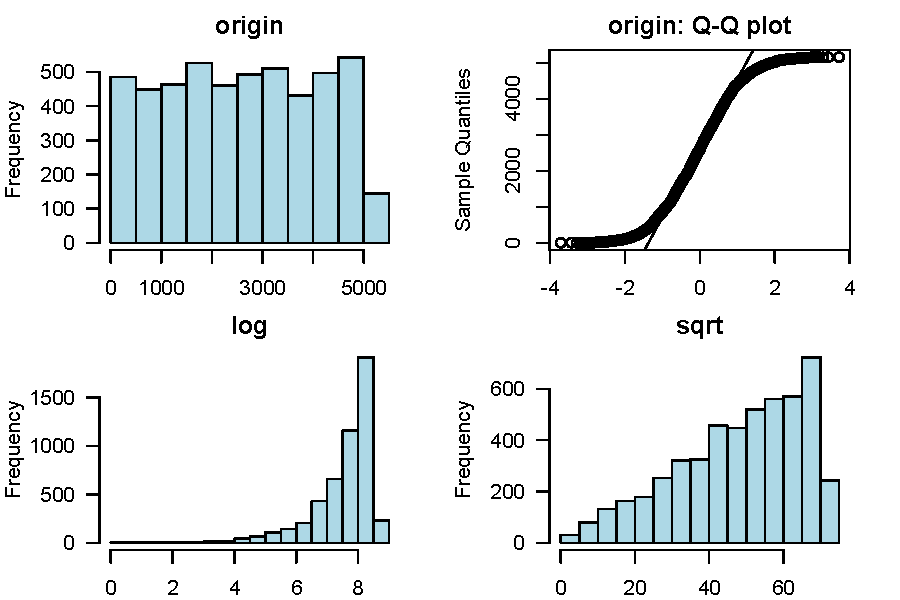
\includegraphics[width=1.0\textwidth]{figure/norm1.pdf}
\caption{idcode}
\end{figure}
\clearpage
\subsubsection{ year }

normality test : Shapiro-Wilk normality test

\noindent statistic : 0.93137,  p-value : 4.35549E-43\\
\\% latex table generated in R 4.0.3 by xtable 1.8-4 package
% Tue Nov 03 00:44:37 2020
\begin{tabular}{lrr}
  \toprule
type & skewness & kurtosis \\ 
  \midrule
original & 0.0820 & 1.6985 \\ 
  log transformation & -0.0030 & 1.6940 \\ 
  sqrt transformation & 0.0395 & 1.6943 \\ 
   \bottomrule
\end{tabular}
\\
\begin{figure}[!ht]
\centering
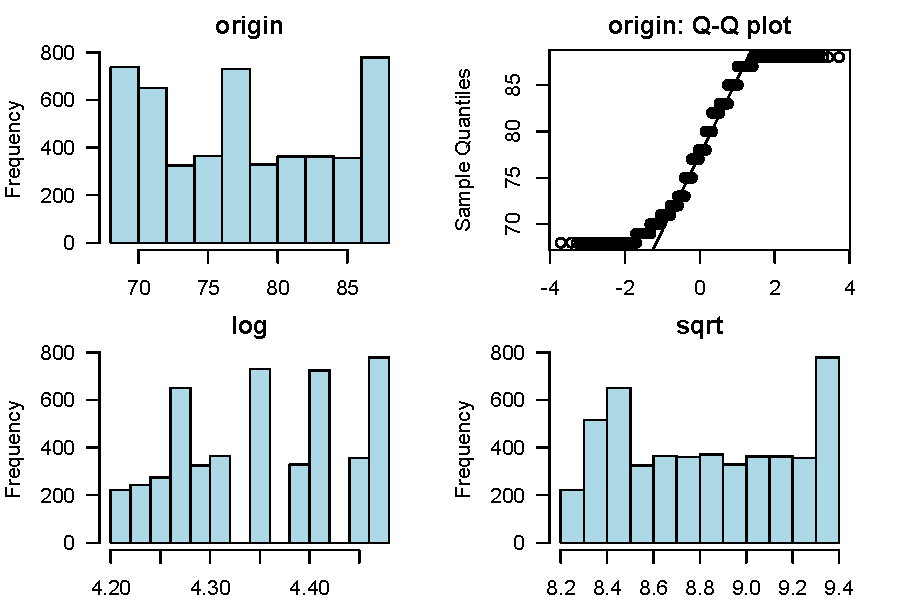
\includegraphics[width=1.0\textwidth]{figure/norm2.pdf}
\caption{year}
\end{figure}
\clearpage
\subsubsection{ birth\_yr }

normality test : Shapiro-Wilk normality test

\noindent statistic : 0.95846,  p-value : 1.41833E-35\\
\\% latex table generated in R 4.0.3 by xtable 1.8-4 package
% Tue Nov 03 00:44:37 2020
\begin{tabular}{lrr}
  \toprule
type & skewness & kurtosis \\ 
  \midrule
original & -0.0959 & 1.9691 \\ 
  log transformation & -0.1889 & 2.0148 \\ 
  sqrt transformation & -0.1422 & 1.9893 \\ 
   \bottomrule
\end{tabular}
\\
\begin{figure}[!ht]
\centering
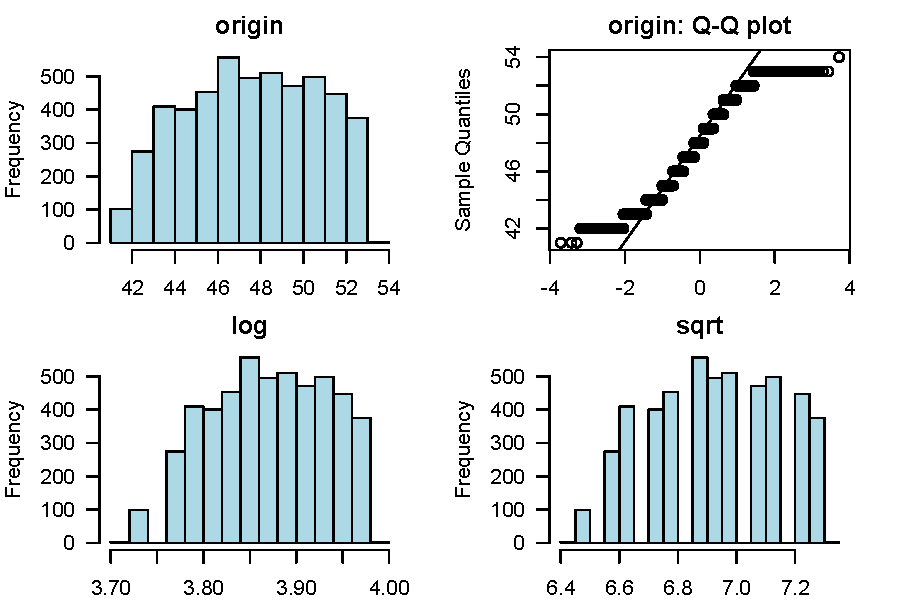
\includegraphics[width=1.0\textwidth]{figure/norm3.pdf}
\caption{birth\_yr}
\end{figure}
\clearpage
\subsubsection{ age }

normality test : Shapiro-Wilk normality test

\noindent statistic : 0.96659,  p-value : 1.51567E-32\\
\\% latex table generated in R 4.0.3 by xtable 1.8-4 package
% Tue Nov 03 00:44:38 2020
\begin{tabular}{lrr}
  \toprule
type & skewness & kurtosis \\ 
  \midrule
original & 0.2548 & 2.0586 \\ 
  log transformation & -0.0870 & 1.9937 \\ 
  sqrt transformation & 0.0849 & 1.9855 \\ 
   \bottomrule
\end{tabular}
\\
\begin{figure}[!ht]
\centering
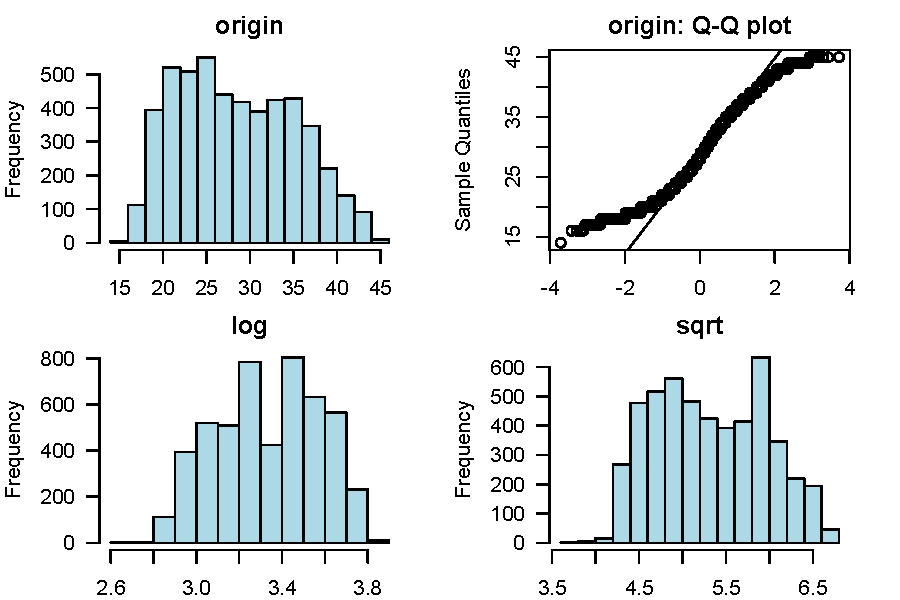
\includegraphics[width=1.0\textwidth]{figure/norm4.pdf}
\caption{age}
\end{figure}
\clearpage
\subsubsection{ msp }

normality test : Shapiro-Wilk normality test

\noindent statistic : 0.62599,  p-value : 5.64809E-74\\
\\% latex table generated in R 4.0.3 by xtable 1.8-4 package
% Tue Nov 03 00:44:38 2020
\begin{tabular}{lrr}
  \toprule
type & skewness & kurtosis \\ 
  \midrule
original & -0.3458 & 1.1196 \\ 
  log transformation &  &  \\ 
  sqrt transformation & -0.3458 & 1.1196 \\ 
   \bottomrule
\end{tabular}
\\
\begin{figure}[!ht]
\centering
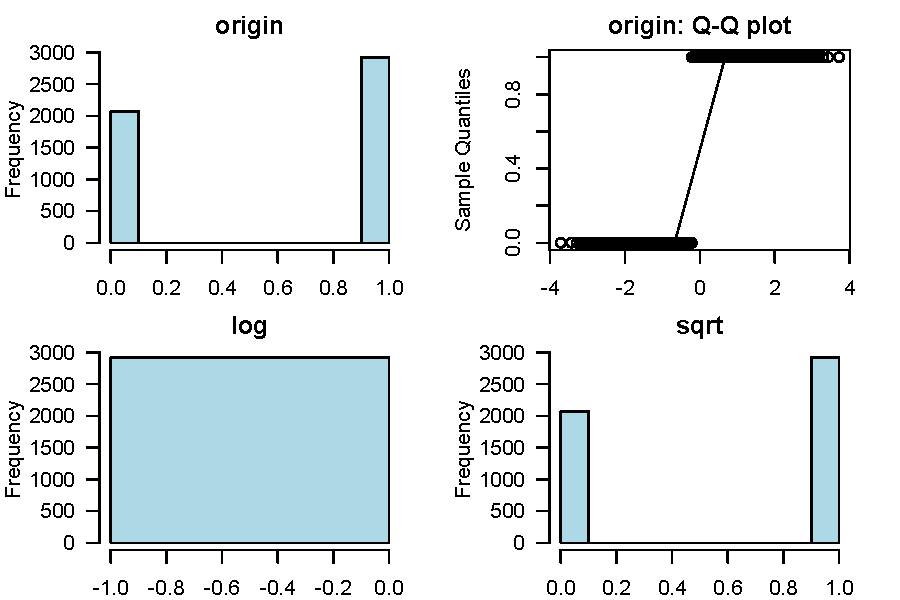
\includegraphics[width=1.0\textwidth]{figure/norm6.pdf}
\caption{msp}
\end{figure}
\clearpage
\subsubsection{ nev\_mar }

normality test : Shapiro-Wilk normality test

\noindent statistic : 0.51937,  p-value : 2.74586E-79\\
\\% latex table generated in R 4.0.3 by xtable 1.8-4 package
% Tue Nov 03 00:44:38 2020
\begin{tabular}{lrr}
  \toprule
type & skewness & kurtosis \\ 
  \midrule
original & 1.2920 & 2.6692 \\ 
  log transformation &  &  \\ 
  sqrt transformation & 1.2920 & 2.6692 \\ 
   \bottomrule
\end{tabular}
\\
\begin{figure}[!ht]
\centering
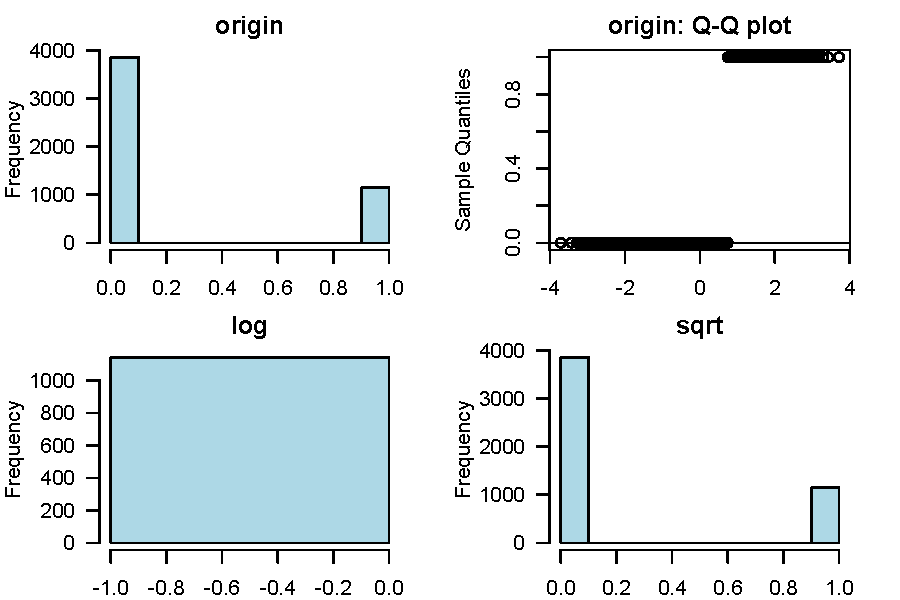
\includegraphics[width=1.0\textwidth]{figure/norm7.pdf}
\caption{nev\_mar}
\end{figure}
\clearpage
\subsubsection{ grade }

normality test : Shapiro-Wilk normality test

\noindent statistic : 0.88882,  p-value : 5.25145E-51\\
\\% latex table generated in R 4.0.3 by xtable 1.8-4 package
% Tue Nov 03 00:44:38 2020
\begin{tabular}{lrr}
  \toprule
type & skewness & kurtosis \\ 
  \midrule
original & 0.0831 & 4.4863 \\ 
  log transformation &  &  \\ 
  sqrt transformation & -1.2718 & 15.0690 \\ 
   \bottomrule
\end{tabular}
\\
\begin{figure}[!ht]
\centering
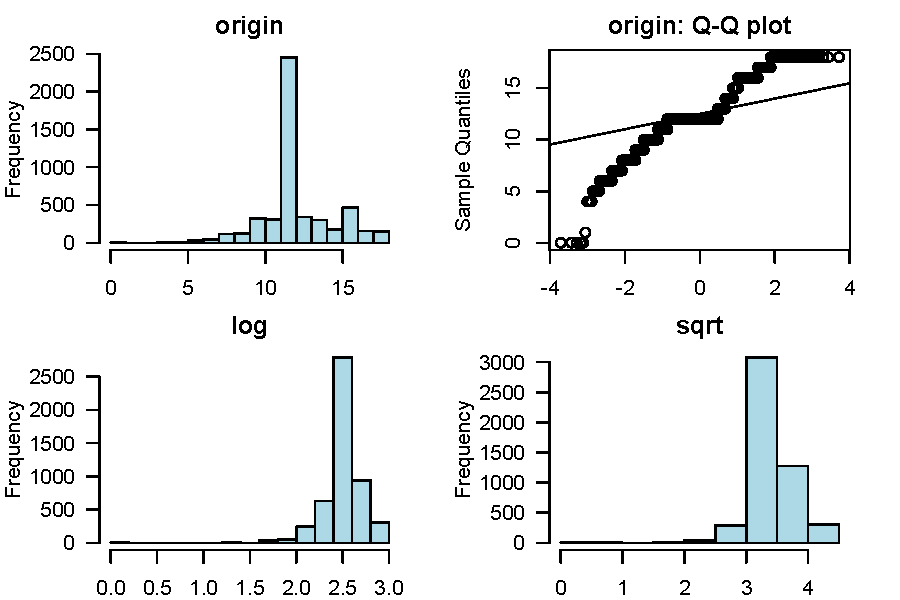
\includegraphics[width=1.0\textwidth]{figure/norm8.pdf}
\caption{grade}
\end{figure}
\clearpage
\subsubsection{ collgrad }

normality test : Shapiro-Wilk normality test

\noindent statistic : 0.45407,  p-value : 4.63132E-82\\
\\% latex table generated in R 4.0.3 by xtable 1.8-4 package
% Tue Nov 03 00:44:38 2020
\begin{tabular}{lrr}
  \toprule
type & skewness & kurtosis \\ 
  \midrule
original & 1.7551 & 4.0806 \\ 
  log transformation &  &  \\ 
  sqrt transformation & 1.7551 & 4.0806 \\ 
   \bottomrule
\end{tabular}
\\
\begin{figure}[!ht]
\centering
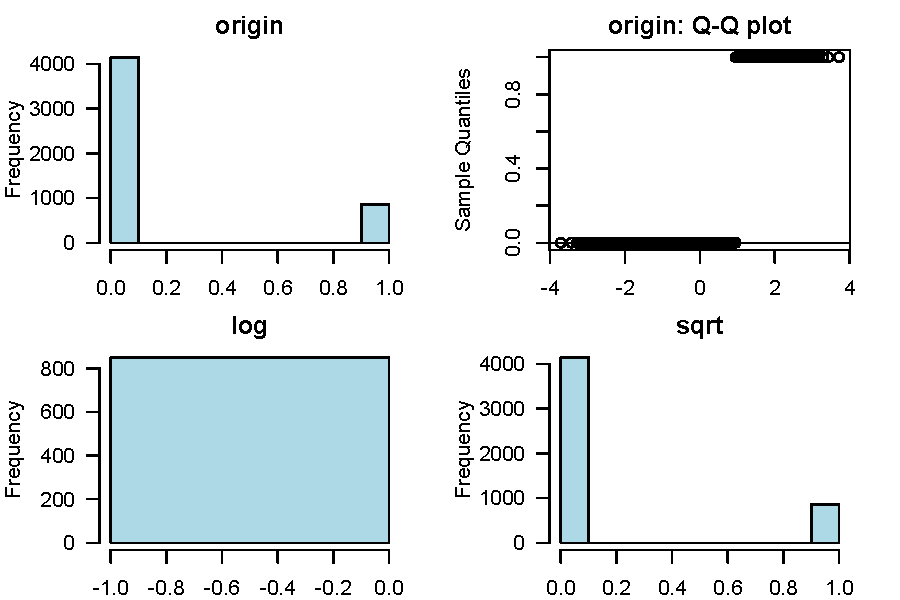
\includegraphics[width=1.0\textwidth]{figure/norm9.pdf}
\caption{collgrad}
\end{figure}
\clearpage
\subsubsection{ not\_smsa }

normality test : Shapiro-Wilk normality test

\noindent statistic : 0.56419,  p-value : 3.42199E-77\\
\\% latex table generated in R 4.0.3 by xtable 1.8-4 package
% Tue Nov 03 00:44:38 2020
\begin{tabular}{lrr}
  \toprule
type & skewness & kurtosis \\ 
  \midrule
original & 0.9636 & 1.9286 \\ 
  log transformation &  &  \\ 
  sqrt transformation & 0.9636 & 1.9286 \\ 
   \bottomrule
\end{tabular}
\\
\begin{figure}[!ht]
\centering
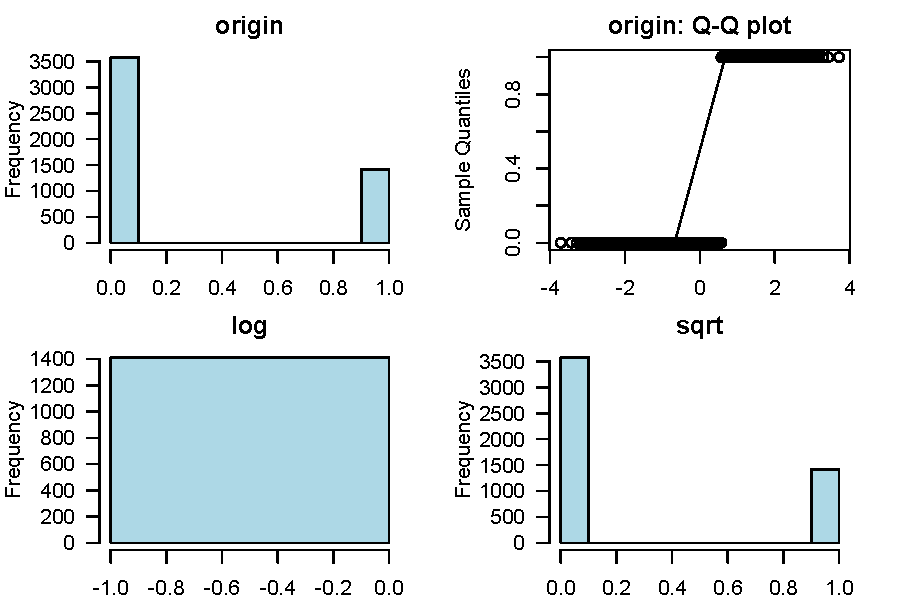
\includegraphics[width=1.0\textwidth]{figure/norm10.pdf}
\caption{not\_smsa}
\end{figure}
\clearpage
\subsubsection{ c\_city }

normality test : Shapiro-Wilk normality test

\noindent statistic : 0.60379,  p-value : 3.36566E-75\\
\\% latex table generated in R 4.0.3 by xtable 1.8-4 package
% Tue Nov 03 00:44:39 2020
\begin{tabular}{lrr}
  \toprule
type & skewness & kurtosis \\ 
  \midrule
original & 0.6216 & 1.3864 \\ 
  log transformation &  &  \\ 
  sqrt transformation & 0.6216 & 1.3864 \\ 
   \bottomrule
\end{tabular}
\\
\begin{figure}[!ht]
\centering
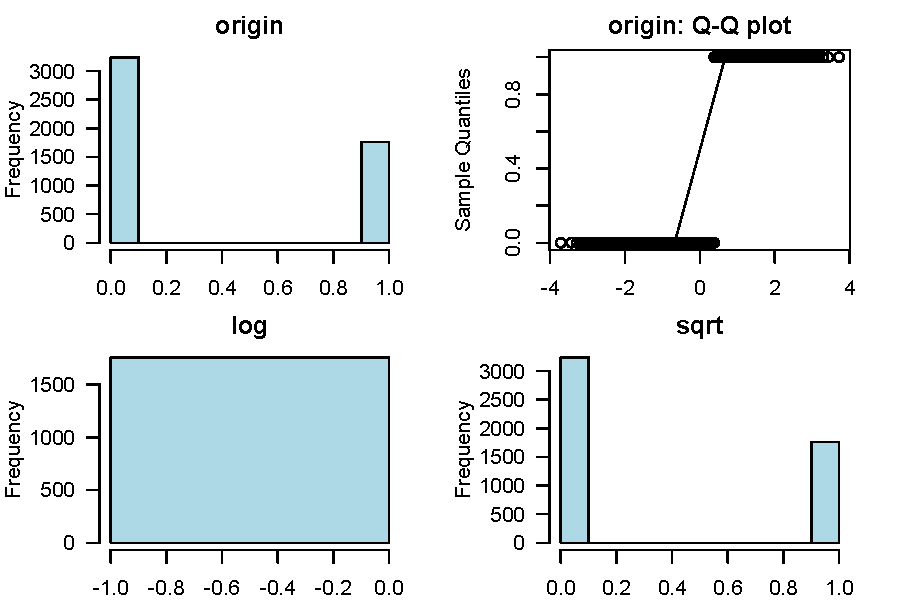
\includegraphics[width=1.0\textwidth]{figure/norm11.pdf}
\caption{c\_city}
\end{figure}
\clearpage
\subsubsection{ south }

normality test : Shapiro-Wilk normality test

\noindent statistic : 0.62577,  p-value : 5.32357E-74\\
\\% latex table generated in R 4.0.3 by xtable 1.8-4 package
% Tue Nov 03 00:44:39 2020
\begin{tabular}{lrr}
  \toprule
type & skewness & kurtosis \\ 
  \midrule
original & 0.3493 & 1.1220 \\ 
  log transformation &  &  \\ 
  sqrt transformation & 0.3493 & 1.1220 \\ 
   \bottomrule
\end{tabular}
\\
\begin{figure}[!ht]
\centering
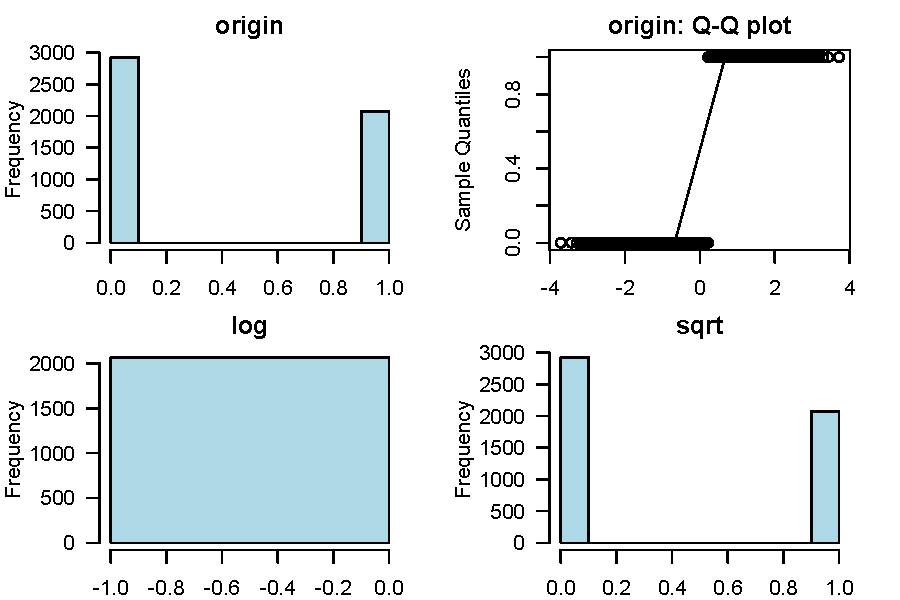
\includegraphics[width=1.0\textwidth]{figure/norm12.pdf}
\caption{south}
\end{figure}
\clearpage
\subsubsection{ ind\_code }

normality test : Shapiro-Wilk normality test

\noindent statistic : 0.8753,  p-value : 8.57421E-53\\
\\% latex table generated in R 4.0.3 by xtable 1.8-4 package
% Tue Nov 03 00:44:39 2020
\begin{tabular}{lrr}
  \toprule
type & skewness & kurtosis \\ 
  \midrule
original & -0.0070 & 1.5784 \\ 
  log transformation & -0.9567 & 4.7754 \\ 
  sqrt transformation & -0.3030 & 2.1755 \\ 
   \bottomrule
\end{tabular}
\\
\begin{figure}[!ht]
\centering
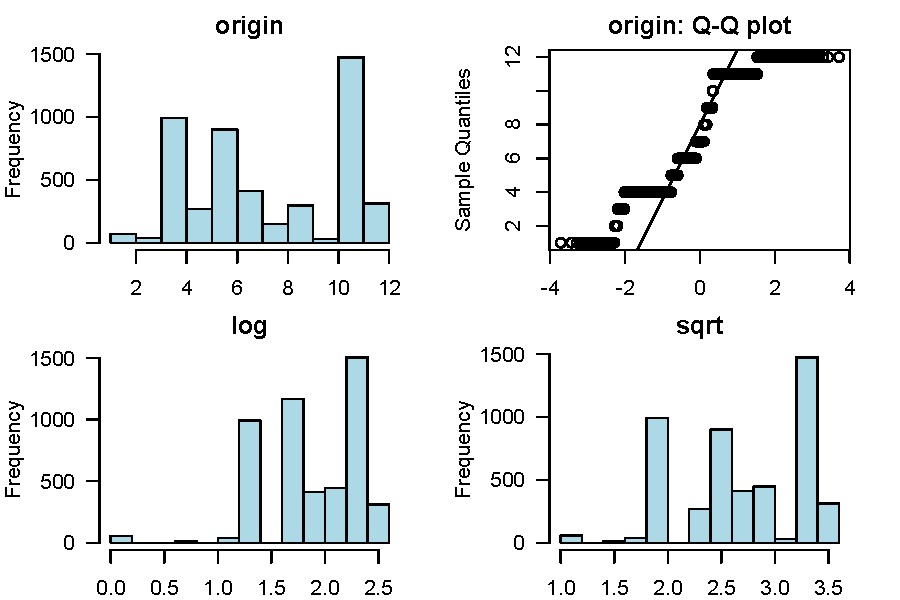
\includegraphics[width=1.0\textwidth]{figure/norm13.pdf}
\caption{ind\_code}
\end{figure}
\clearpage
\subsubsection{ occ\_code }

normality test : Shapiro-Wilk normality test

\noindent statistic : 0.85143,  p-value : 5.09415E-56\\
\\% latex table generated in R 4.0.3 by xtable 1.8-4 package
% Tue Nov 03 00:44:39 2020
\begin{tabular}{lrr}
  \toprule
type & skewness & kurtosis \\ 
  \midrule
original & 1.0923 & 3.6919 \\ 
  log transformation & -0.2909 & 2.6626 \\ 
  sqrt transformation & 0.4553 & 2.6357 \\ 
   \bottomrule
\end{tabular}
\\
\begin{figure}[!ht]
\centering
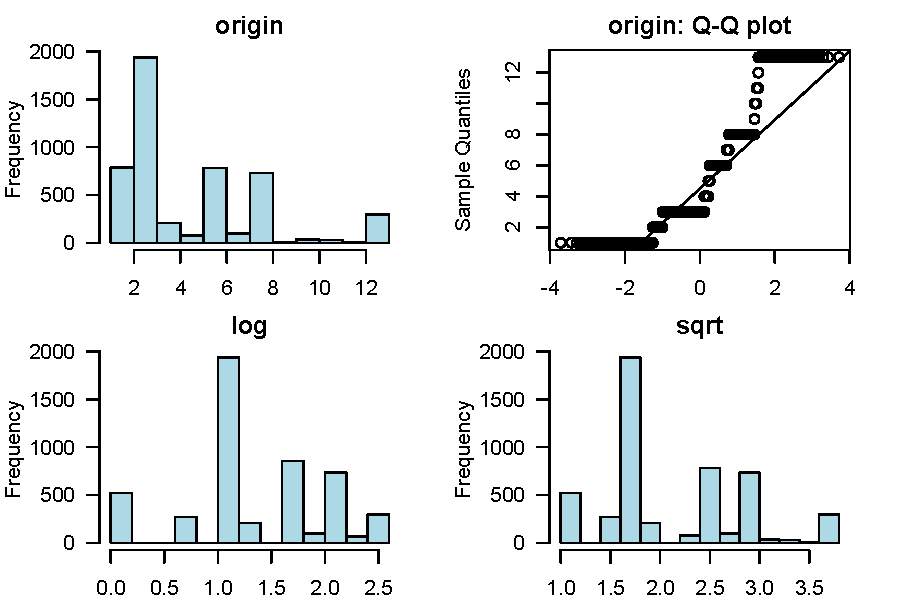
\includegraphics[width=1.0\textwidth]{figure/norm14.pdf}
\caption{occ\_code}
\end{figure}
\clearpage
\subsubsection{ union }

normality test : Shapiro-Wilk normality test

\noindent statistic : 0.51696,  p-value : 1.01762E-70\\
\\% latex table generated in R 4.0.3 by xtable 1.8-4 package
% Tue Nov 03 00:44:39 2020
\begin{tabular}{lrr}
  \toprule
type & skewness & kurtosis \\ 
  \midrule
original & 1.3090 & 2.7134 \\ 
  log transformation &  &  \\ 
  sqrt transformation & 1.3090 & 2.7134 \\ 
   \bottomrule
\end{tabular}
\\
\begin{figure}[!ht]
\centering
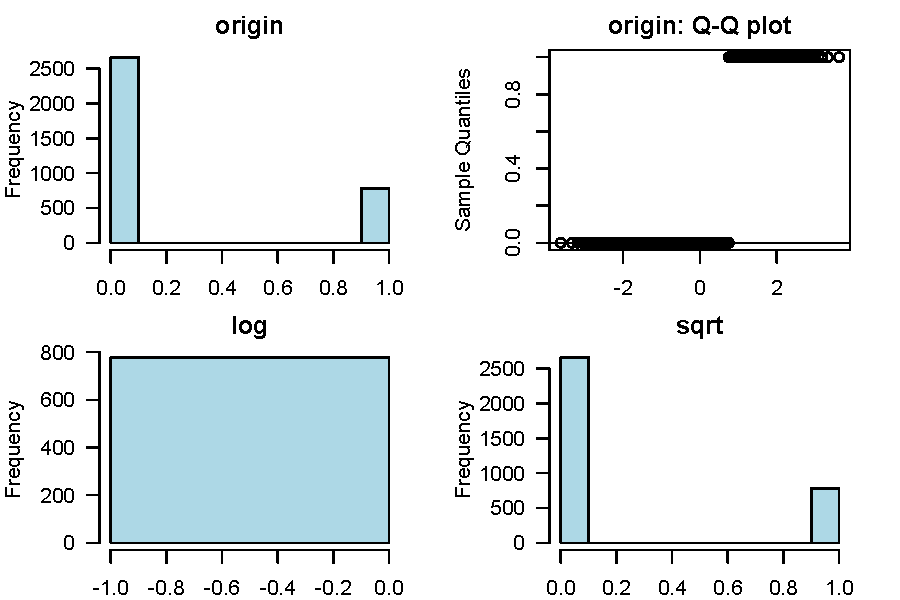
\includegraphics[width=1.0\textwidth]{figure/norm15.pdf}
\caption{union}
\end{figure}
\clearpage
\subsubsection{ wks\_ue }

normality test : Shapiro-Wilk normality test

\noindent statistic : 0.40521,  p-value : 5.40433E-78\\
\\% latex table generated in R 4.0.3 by xtable 1.8-4 package
% Tue Nov 03 00:44:39 2020
\begin{tabular}{lrr}
  \toprule
type & skewness & kurtosis \\ 
  \midrule
original & 3.9695 & 20.6532 \\ 
  log transformation &  &  \\ 
  sqrt transformation & 2.3255 & 7.9054 \\ 
   \bottomrule
\end{tabular}
\\
\begin{figure}[!ht]
\centering
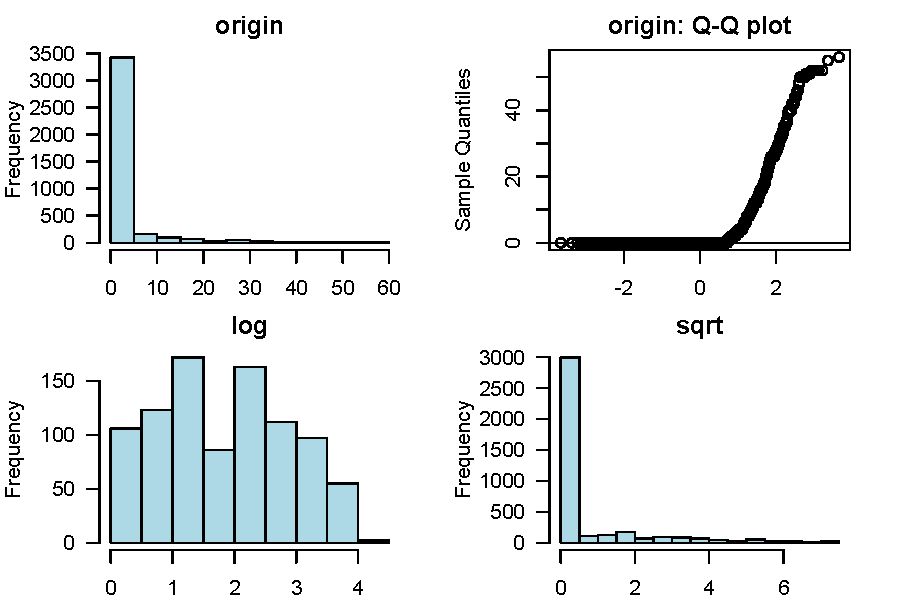
\includegraphics[width=1.0\textwidth]{figure/norm16.pdf}
\caption{wks\_ue}
\end{figure}
\clearpage
\subsubsection{ ttl\_exp }

normality test : Shapiro-Wilk normality test

\noindent statistic : 0.92491,  p-value : 1.6422E-44\\
\\% latex table generated in R 4.0.3 by xtable 1.8-4 package
% Tue Nov 03 00:44:40 2020
\begin{tabular}{lrr}
  \toprule
type & skewness & kurtosis \\ 
  \midrule
original & 0.8811 & 3.1852 \\ 
  log transformation &  &  \\ 
  sqrt transformation & 0.1344 & 2.2991 \\ 
   \bottomrule
\end{tabular}
\\
\begin{figure}[!ht]
\centering
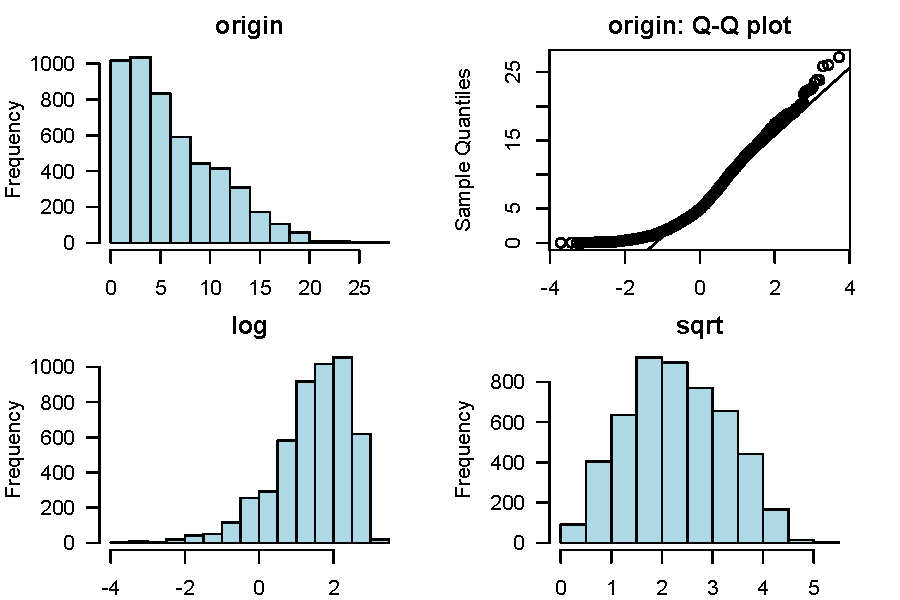
\includegraphics[width=1.0\textwidth]{figure/norm17.pdf}
\caption{ttl\_exp}
\end{figure}
\clearpage
\subsubsection{ tenure }

normality test : Shapiro-Wilk normality test

\noindent statistic : 0.76779,  p-value : 3.76788E-64\\
\\% latex table generated in R 4.0.3 by xtable 1.8-4 package
% Tue Nov 03 00:44:40 2020
\begin{tabular}{lrr}
  \toprule
type & skewness & kurtosis \\ 
  \midrule
original & 1.9097 & 6.7001 \\ 
  log transformation &  &  \\ 
  sqrt transformation & 0.7690 & 3.0527 \\ 
   \bottomrule
\end{tabular}
\\
\begin{figure}[!ht]
\centering
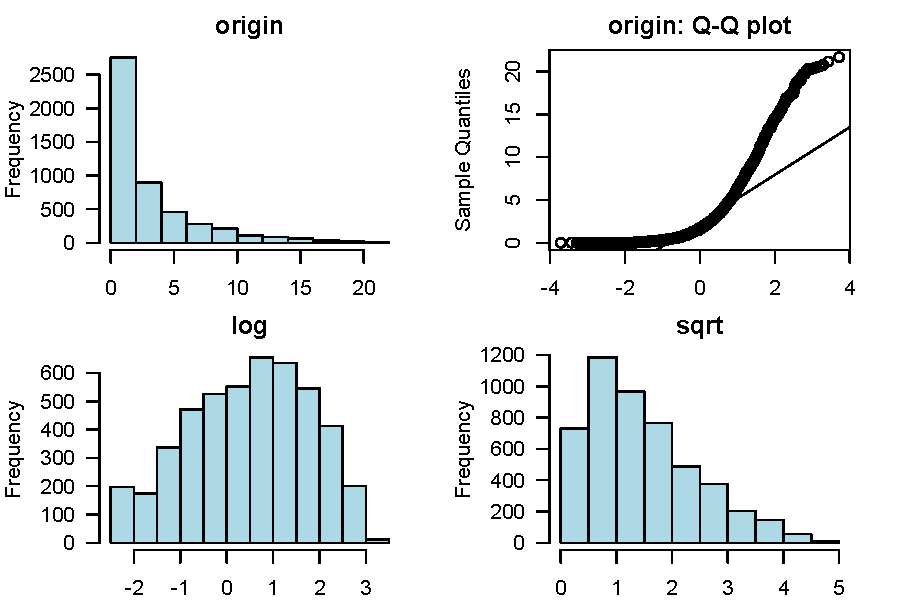
\includegraphics[width=1.0\textwidth]{figure/norm18.pdf}
\caption{tenure}
\end{figure}
\clearpage
\subsubsection{ hours }

normality test : Shapiro-Wilk normality test

\noindent statistic : 0.77474,  p-value : 8.5639E-64\\
\\% latex table generated in R 4.0.3 by xtable 1.8-4 package
% Tue Nov 03 00:44:40 2020
\begin{tabular}{lrr}
  \toprule
type & skewness & kurtosis \\ 
  \midrule
original & -0.3831 & 12.6962 \\ 
  log transformation & -3.1754 & 16.9745 \\ 
  sqrt transformation & -1.7906 & 8.7119 \\ 
   \bottomrule
\end{tabular}
\\
\begin{figure}[!ht]
\centering
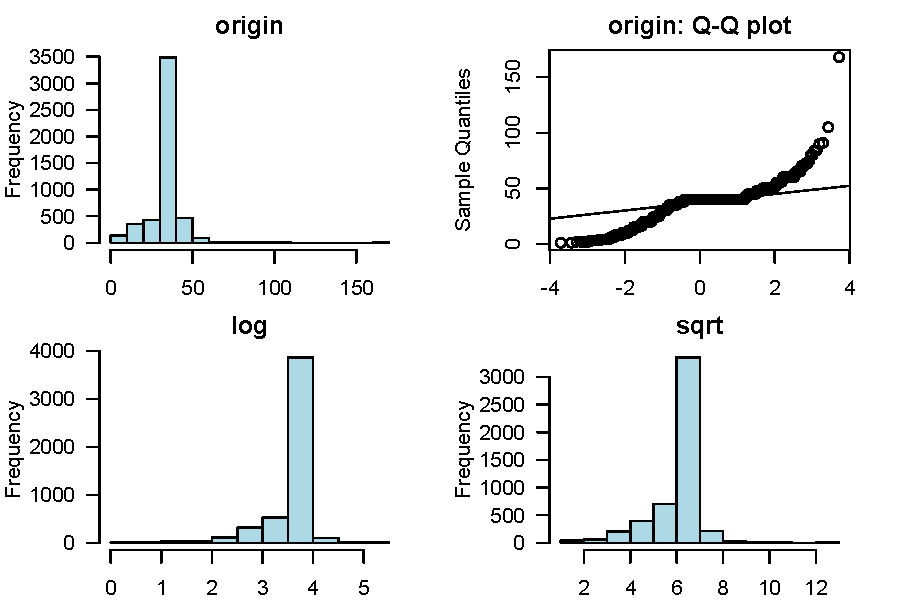
\includegraphics[width=1.0\textwidth]{figure/norm19.pdf}
\caption{hours}
\end{figure}
\clearpage
\subsubsection{ wks\_work }

normality test : Shapiro-Wilk normality test

\noindent statistic : 0.9383,  p-value : 5.19531E-41\\
\\% latex table generated in R 4.0.3 by xtable 1.8-4 package
% Tue Nov 03 00:44:40 2020
\begin{tabular}{lrr}
  \toprule
type & skewness & kurtosis \\ 
  \midrule
original & 0.1933 & 2.3432 \\ 
  log transformation &  &  \\ 
  sqrt transformation & -0.7641 & 3.5887 \\ 
   \bottomrule
\end{tabular}
\\
\begin{figure}[!ht]
\centering
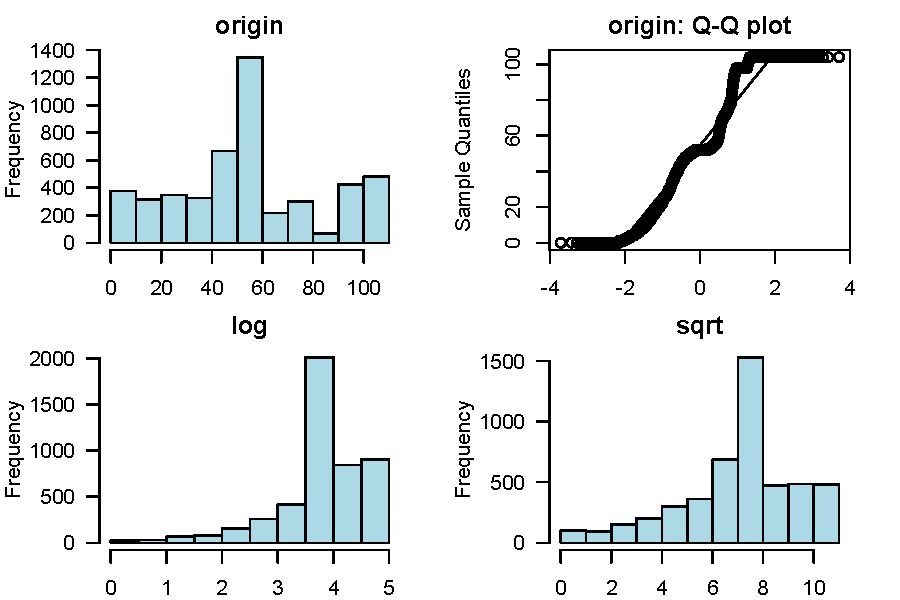
\includegraphics[width=1.0\textwidth]{figure/norm20.pdf}
\caption{wks\_work}
\end{figure}
\clearpage
\subsubsection{ ln\_wage }

normality test : Shapiro-Wilk normality test

\noindent statistic : 0.97666,  p-value : 7.08836E-28\\
\\% latex table generated in R 4.0.3 by xtable 1.8-4 package
% Tue Nov 03 00:44:40 2020
\begin{tabular}{lrr}
  \toprule
type & skewness & kurtosis \\ 
  \midrule
original & 0.3992 & 4.8522 \\ 
  log transformation & -3.4099 & 29.2277 \\ 
  sqrt transformation & -0.6972 & 6.6385 \\ 
   \bottomrule
\end{tabular}
\\
\begin{figure}[!ht]
\centering
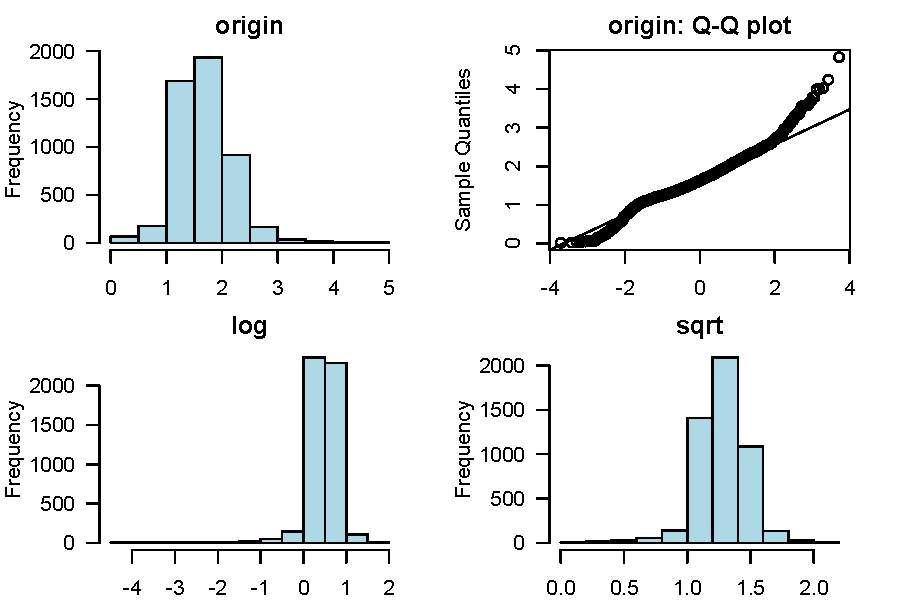
\includegraphics[width=1.0\textwidth]{figure/norm21.pdf}
\caption{ln\_wage}
\end{figure}
\clearpage

\chapter{Relationship Between Variables}
\section{Correlation Coefficient}
\subsection{Correlation Coefficient by Variable Combination}

\begin{longtable}[t]{llr}
\caption{\label{tab:correlations}The correlation coefficients (0.5 or more)}\\
\toprule
Variable1 & Variable2 & Correlation Coefficient\\
\midrule
\endfirsthead
\caption[]{The correlation coefficients (0.5 or more) \textit{(continued)}}\\
\toprule
Variable1 & Variable2 & Correlation Coefficient\\
\midrule
\endhead

\endfoot
\bottomrule
\endlastfoot
\cellcolor{gray!6}{age} & \cellcolor{gray!6}{year} & \cellcolor{gray!6}{0.895}\\
ttl\_exp & year & 0.777\\
\cellcolor{gray!6}{collgrad} & \cellcolor{gray!6}{grade} & \cellcolor{gray!6}{0.757}\\
ttl\_exp & age & 0.756\\
\cellcolor{gray!6}{tenure} & \cellcolor{gray!6}{ttl\_exp} & \cellcolor{gray!6}{0.674}\\
\addlinespace
nev\_mar & msp & -0.673\\
\cellcolor{gray!6}{wks\_work} & \cellcolor{gray!6}{ttl\_exp} & \cellcolor{gray!6}{0.630}\\
wks\_work & year & 0.565\\
\cellcolor{gray!6}{wks\_work} & \cellcolor{gray!6}{age} & \cellcolor{gray!6}{0.525}\\*
\end{longtable}

\subsection{Correlation Plot of Numerical Variables}
\begin{figure}[!ht]
\centering
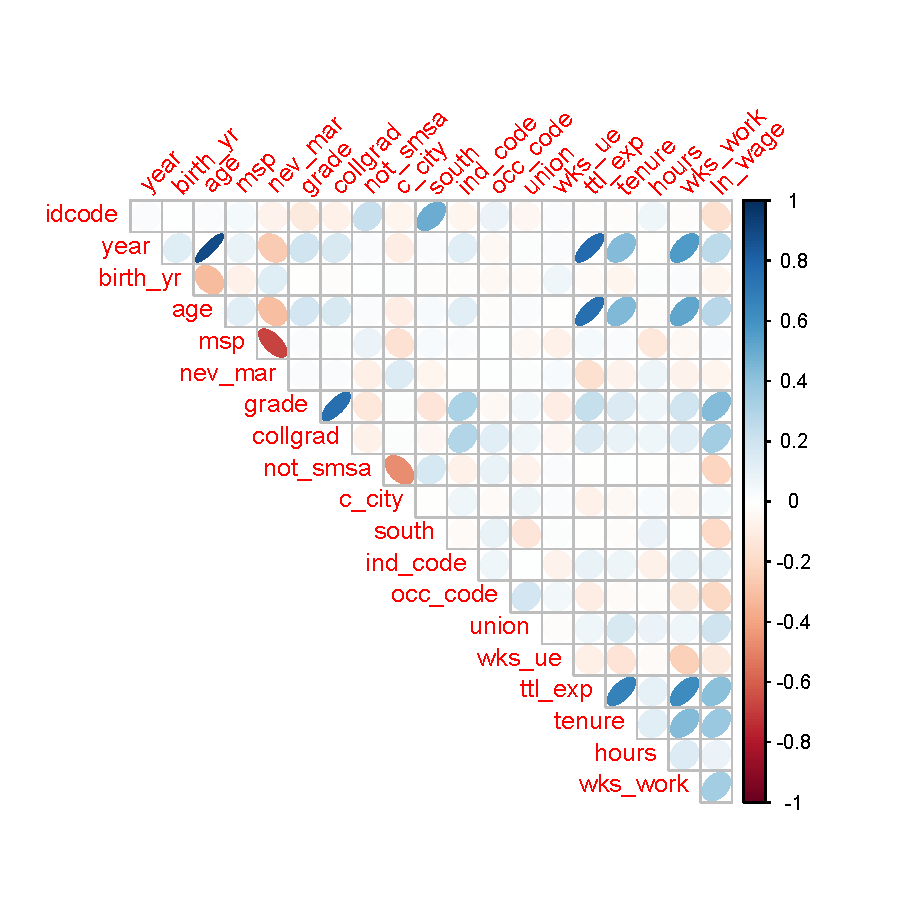
\includegraphics[width=0.99\textwidth]{figure/correlation.pdf}
\caption{The correlation coefficient of numerical variables}
\end{figure}


\chapter{Target based Analysis}
\section{Grouped Descriptive Statistics}
\subsection{Grouped Numerical Variables}

There is no target variable.



\subsection{Grouped Categorical Variables}

There is no target variable.



\section{Grouped Relationship Between Variables}
\subsection{Grouped Correlation Coefficient}
There is no target variable.



\subsection{Grouped Correlation Plot of Numerical Variables}
There is no target variable.






\end{document}
